
\chapter{Fundamentação Teórica} \label{cap:FundamentacaoTeorica}


\section{Digitalização industrial e transformação digital}

A digitalização industrial pode ser compreendida como a conversão de atividades, registros e fluxos de informação, antes realizados de forma manual ou analógica, para meios digitais. No contexto da manufatura, essa mudança favorece a rastreabilidade, reduz limitações associadas ao preenchimento manual e facilita o acompanhamento das operações produtivas \cite{leite2024}.

A Transformação Digital (TD) possui um escopo mais amplo, pois envolve alterações nos processos, na estrutura organizacional e nas formas de gestão a partir do uso de tecnologias digitais \cite{murici2022}. Nesse sentido, a digitalização de processos industriais pode ser entendida como uma aplicação prática da TD no chão de fábrica, sobretudo quando orientada à melhoria da eficiência operacional, da qualidade e da tomada de decisão \cite{sanchis2020,ribeiro2026}.

\section{Indústria 4.0 e dados no ambiente de manufatura}

A Indústria 4.0 caracteriza-se pela integração de tecnologias digitais aos processos produtivos, possibilitando maior conexão entre máquinas, sistemas, pessoas e dispositivos. Nesse cenário, os dados assumem papel estratégico, pois apoiam o acompanhamento das operações, a análise de desempenho e a tomada de decisão, contribuindo para maior controle dos processos industriais \cite{sanchis2020,ribeiro2026}.

No contexto fabril, esses dados podem surgir de registros de produção, apontamentos operacionais, inspeções de qualidade, tempos de execução, ocorrências de falhas e informações coletadas por equipamentos conectados. Como observa \citeonline{rogers2016}, os dados podem ser gerados nas atividades internas da organização, como manufatura e operações, e utilizados em avaliações, previsões e decisões. Além disso, \citeonline{sanchis2020} associam o ambiente manufatureiro conectado à comunicação entre pessoas, aplicações e dispositivos de Internet das Coisas, o que amplia a disponibilidade e o uso dessas informações no processo produtivo.

A Transformação Digital 4.0, portanto, não depende apenas da adoção de ferramentas tecnológicas, mas também de condições organizacionais que sustentem o uso dos dados. \citeonline{leite2024} destacam dimensões como cultura digital, gestão da informação, infraestrutura tecnológica, operações estruturadas e desenvolvimento de competências digitais. Conforme a Figura~\ref{fig:dimensoes-td40}, esses elementos ajudam a visualizar como a digitalização industrial articula tecnologia, capacidade organizacional e uso das informações geradas no chão de fábrica.

\begin{figure}[htb]
    \centering
    \caption{Dimensões base para a Transformação Digital 4.0}
    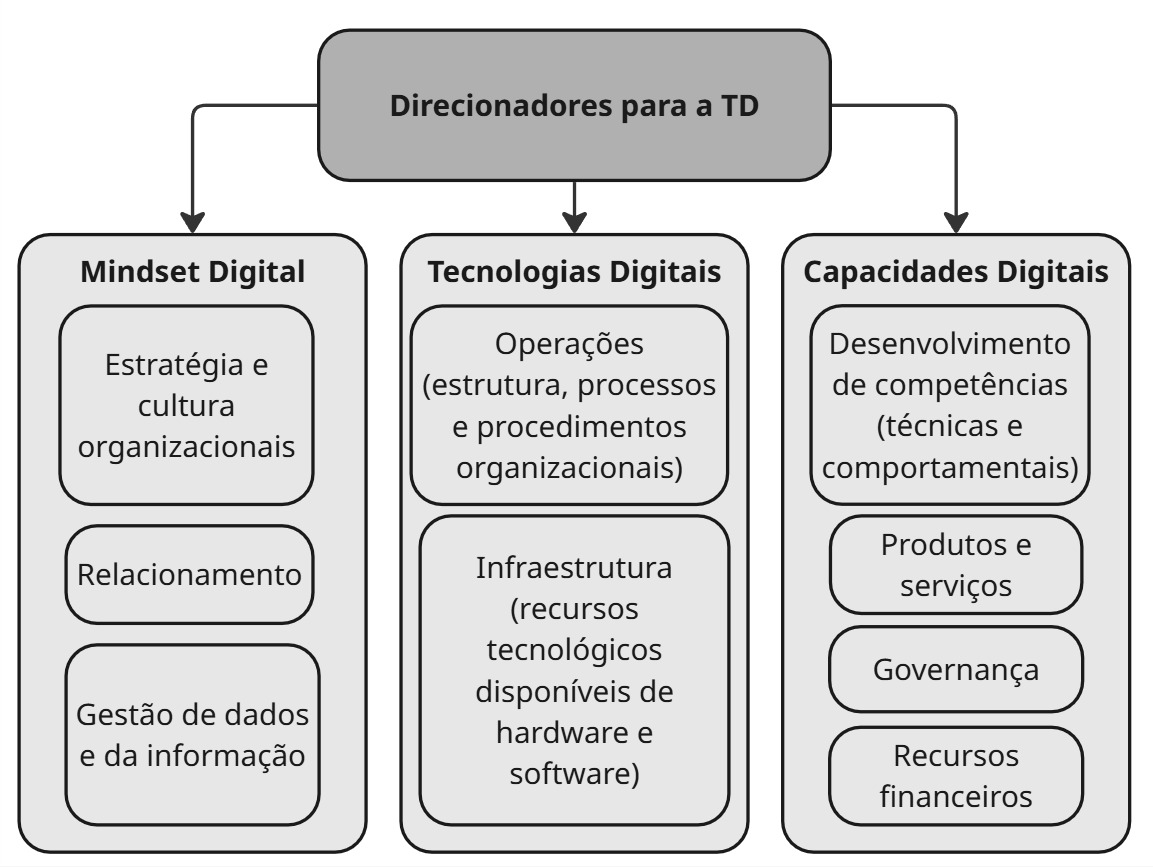
\includegraphics[width=0.85\textwidth]{Figuras/direcionadores_td.jpg}
    \label{fig:dimensoes-td40}
    
    \vspace{0.2cm}
    \begin{flushleft}
    \footnotesize Fonte: Elaborada pelo autor, com base em \citeonline{leite2024}.
    \end{flushleft}
\end{figure}

\section{Ferramentas low-code aplicadas à indústria}

As ferramentas \textit{low-code} podem ser compreendidas como plataformas de desenvolvimento que permitem a criação de aplicações digitais com menor dependência de codificação manual. Segundo \citeonline{sanchis2020}, essas plataformas utilizam interfaces visuais e componentes previamente estruturados, favorecendo o desenvolvimento rápido de aplicações. De forma complementar, \citeonline{alves2022} destacam que essa abordagem se apoia em abstrações de alto nível, diagramas visuais e linguagens declarativas, possibilitando menores tempos e custos quando comparada aos modelos tradicionais de desenvolvimento.

Na indústria, essa abordagem torna-se relevante por permitir que soluções digitais sejam desenvolvidas de forma mais flexível e próxima das demandas operacionais. Aplicações como formulários digitais, fluxos de aprovação, painéis de acompanhamento e integrações entre etapas produtivas podem ser construídas com maior agilidade. Com isso, o \textit{low-code} contribui para adaptar as soluções às rotinas do chão de fábrica e aos requisitos dos usuários envolvidos na operação \cite{sanchis2020,alves2022}.

Outro aspecto importante é a aproximação entre as áreas de negócio, processos e Tecnologia da Informação (TI). \citeonline{alves2022} apontam que o \textit{low-code} favorece a participação de profissionais que conhecem diretamente os procedimentos, desde a concepção até a validação das aplicações. Essa participação tende a gerar soluções mais aderentes à rotina operacional, especialmente em ambientes industriais nos quais o conhecimento prático do processo é essencial para definir fluxos, requisitos e informações necessárias.

Ao analisar plataformas \textit{low-code} de destaque, \citeonline{alves2022} comparam seus principais pontos fortes e limitações. Essa análise é relevante para este trabalho porque mostra que a escolha de uma plataforma não deve considerar apenas a rapidez de desenvolvimento, mas também aspectos como integração com sistemas existentes, colaboração entre usuários, gestão de fluxos, escalabilidade, manutenção e suporte a testes. O Quadro~\ref{quad:comparacao-lowcode} apresenta uma adaptação dessa comparação, relacionando características importantes para aplicações industriais.

\begin{quadro}[htb]
\centering
\caption{Comparação entre plataformas \textit{low-code}}
\label{quad:comparacao-lowcode}
\footnotesize
\begin{tabularx}{\textwidth}{>{\raggedright\arraybackslash}p{2.8cm}
                                >{\raggedright\arraybackslash}X
                                >{\raggedright\arraybackslash}X}
\hline
\textbf{Plataforma} & \textbf{Pontos fortes} & \textbf{Pontos de atenção} \\
\hline

Power Apps &
Integração com serviços em nuvem, uso de APIs personalizadas, suporte à política de dados, colaboração entre usuários e automação de fluxos de trabalho. &
Licenciamento complexo, menor suporte para desenvolvedores profissionais e restrições para compartilhamento externo. \\

\hline

OutSystems &
Boa experiência de usuário, escalabilidade, análise de desempenho e interoperabilidade. &
Poucos conectores externos, baixo suporte a estruturas de testes e ausência de desenvolvimento \textit{off-line}. \\

\hline

Mendix &
Suporte móvel \textit{off-line}, gerenciamento ágil de projetos, colaboração entre usuários e variedade de opções de implantação. &
Baixa integração com sistemas ERP, possíveis inconsistências em novas versões e custo elevado. \\

\hline

Salesforce Lightning &
Escalabilidade, recursos de teste, ferramentas associadas à inteligência artificial, gerenciamento amigável e serviço robusto. &
Possíveis instabilidades em integrações, maior necessidade de treinamento e menor nível de automação. \\

\hline

Appian &
Histórico agregado de processos, processamento de eventos complexos, colaboração simultânea, interfaces intuitivas e implantação rápida. &
Personalização limitada, depuração mais demorada e baixo suporte para testes. \\

\hline
\end{tabularx}

\vspace{0.2cm}
\begin{flushleft}
\footnotesize Fonte: Adaptado de \citeonline[p.~7--8]{alves2022}.
\end{flushleft}
\end{quadro}

O quadro reforça que as plataformas \textit{low-code} possuem características favoráveis à digitalização de processos industriais, principalmente quando o objetivo é transformar fluxos operacionais em aplicações digitais de uso prático. Para este estudo, destacam-se os recursos de integração, colaboração, automação de fluxos e disponibilização rápida das aplicações. Ao mesmo tempo, \citeonline{sanchis2020} chama atenção para desafios como escalabilidade, fragmentação entre plataformas e adequação a aplicações mais complexas. Assim, a adoção do \textit{low-code} deve ser acompanhada por análise do processo, validação com os usuários, acompanhamento das soluções implementadas e definição de critérios de governança \cite{sanchis2020,alves2022}.



\section{Aplicação digitalizada no estudo de caso}

\subsection{\textit{Resposta rápida para o controle da qualidade: 
conceito, funcionamento e aplicação}}

A Resposta Rápida para o Controle da Qualidade, conhecida pela sigla QRQC, do inglês \textit{Quick Response to Quality Control}, é utilizada para tratar problemas de qualidade de forma estruturada, com foco na reação rápida, na contenção do desvio, na análise da causa e na definição de ações corretivas capazes de evitar a reincidência da falha. Segundo \citeonline{rocha2012}, o QRQC é uma metodologia de gerenciamento à vista que reúne ferramentas da qualidade para apoiar a análise e a identificação de problemas no processo produtivo.

A aplicação do QRQC está associada à necessidade de resolver problemas diretamente na fonte, com base em fatos, evidências e participação dos envolvidos no processo. Para \citeonline{rocha2012}, a metodologia utiliza ferramentas como 5W2H, Diagrama de Ishikawa, 5 Porquês e Diagrama de Pareto, aplicadas de forma sequencial para auxiliar na contenção do problema e na investigação das causas. Dessa forma, o QRQC contribui para organizar a tratativa das não conformidades e tornar mais clara a relação entre o problema identificado, suas causas e as ações necessárias.

O funcionamento da metodologia pode ser compreendido como um fluxo de resposta rápida que começa pela identificação do problema e pela adoção de ações imediatas de contenção. Em seguida, são analisados os riscos de ocorrência em outros produtos ou processos, investigadas as causas da falha e da não detecção, definidas ações corretivas e verificada a efetividade das soluções adotadas. \citeonline{moreira2023} relaciona essa lógica às etapas da metodologia 8D, envolvendo definição do problema, análise de risco, contenção, identificação das causas, ações corretivas, verificação e registro das lições aprendidas.

No ambiente industrial, a aplicação do QRQC depende da integração entre pessoas, registros e informações do processo. A participação dos colaboradores que atuam diretamente na operação é importante porque permite que a análise considere o local real da ocorrência, as condições do processo e as evidências disponíveis. Nesse sentido, \citeonline{moreira2023} destaca que o comprometimento dos envolvidos e da gestão é essencial para que a metodologia contribua para a melhoria contínua e para o tratamento adequado dos problemas de qualidade.

No contexto deste estudo, o QRQC é as aplicação digitalizada porque envolve informações que precisam ser registradas, acompanhadas e atualizadas ao longo da tratativa da não conformidade. Entre essas informações, podem estar a descrição do problema, a área responsável, as ações de contenção, os prazos, os responsáveis, as evidências, as causas identificadas e a verificação da eficácia das ações. Assim, a digitalização desse processo pode apoiar a rastreabilidade das ocorrências, a padronização dos registros e o acompanhamento das ações em andamento, aproximando a metodologia de resposta rápida das práticas de gestão da informação no ambiente de manufatura.


\section{Barreiras e cuidados na digitalização de processos industriais}

A digitalização de processos industriais pode contribuir para a organização das informações, o acompanhamento das atividades e a tomada de decisão. No entanto, sua implantação exige cuidados que vão além da escolha da ferramenta tecnológica. \citeonline{murici2022} destaca que a Transformação Digital envolve mudanças em processos, estrutura, cultura, competências e formas de gestão, o que evidencia a necessidade de considerar também os fatores humanos e organizacionais.

Entre as principais barreiras, estão a resistência à mudança, a carência de pessoal qualificado, o despreparo dos usuários e a dificuldade de adaptação a novos fluxos de trabalho \cite{murici2022}. No ambiente de manufatura, esses fatores podem interferir diretamente no uso das aplicações digitais, especialmente quando há substituição de registros manuais por formulários eletrônicos, necessidade de padronização dos dados e acompanhamento das informações em tempo real.

Também devem ser considerados aspectos técnicos e de governança. Embora as plataformas \textit{low-code} favoreçam o desenvolvimento rápido de aplicações, \citeonline{sanchis2020} apontam desafios relacionados à escalabilidade, fragmentação entre plataformas e adequação a aplicações mais complexas. Dessa forma, a digitalização de processos industriais deve ser acompanhada por análise do processo, validação com os usuários, definição de responsabilidades, controle dos dados e manutenção das soluções implementadas \cite{alves2022}.






% \section{Acrescentando um arquivo tex na estrutura}

Como acrescentar uma nova subseção, utilizando um arquivo externo:

\begin{enumerate}
    \item crie um arquivo .tex (ex.: meuarquivo.tex)
    \item Se for um arquivo de capítulo:
        \subitem No arquivo Monografia.text acrescente a seguinte linha na ordem que deseja aparecer no texto: $\backslash include\{Capitulos/meuarquivo\}$
    \item Se for parte do texto:
        \subitem Inserir no arquivo onde se deseja continuar o seguinte comando:
            \subsubitem $\backslash input\{Capitulos/meuarquivo\}$
    
    
\end{enumerate}


{\color{blue}

Obs.: Este texto foi escrito no arquivo exemplo subsecao2.tex. 
Note que o arquivo é inserido em continuidade na página!

}
 % a ordem é a que aparece no texto





